
\documentclass[a4paper,11pt]{article}
\usepackage[T1]{fontenc}
\usepackage[utf8]{inputenc}
\usepackage{lmodern}
\usepackage{hyperref}
\usepackage{graphicx}
\usepackage[english]{babel}
\newenvironment{dedication}
{
   \cleardoublepage
   \thispagestyle{empty}
   \vspace*{\stretch{1}}
   \hfill\begin{minipage}[t]{0.66\textwidth}
   \raggedright
}
{
   \end{minipage}
   \vspace*{\stretch{3}}
   \clearpage
}

\makeatletter
%\renewcommand{\@chapapp}{}% Not necessary...
\newenvironment{chapquote}[2][2em]
  {\setlength{\@tempdima}{#1}%
   \def\chapquote@author{#2}%
   \parshape 1 \@tempdima \dimexpr\textwidth-2\@tempdima\relax%
   \itshape}
  {\par\normalfont\hfill--\ \chapquote@author\hspace*{\@tempdima}\par\bigskip}
\makeatother
\title{\Huge \textbf{\v{S}ifrovanje elektronske po\v{s}te: Windows}}

\author{\textsc{Cryptoparty Serbia}}
\begin{document}


%\frontmatter
\maketitle
\tableofcontents

%\mainmatter
\newpage
\section{Kratak uvod}
Ovo uputstvo \'{c}e vam pokazati kako da \v{s}ifrujete elektronsku po\v{s}tu na operativnom sistemu Windows koriste\'{c}i \textbf{Thunderbird} klijenta elektronske po\v{s}te tj. imejl klijenta.

\section{Instalacija Gpg4win programa}
Od softvera su nam potrebni \textbf{Gpg4win} program koji barata sa procesom \v{s}ifrovanja, de\v{s}ifrovanja, digitalnog potpisivanja i provere digitalnog potpisa.
\newline \textbf{Gpg4win} mo\v{z}ete preuzeti sa \href{http://www.gpg4win.org}{www.gpg4win.org}


\begin{figure}[!h]
	\begin{center}
		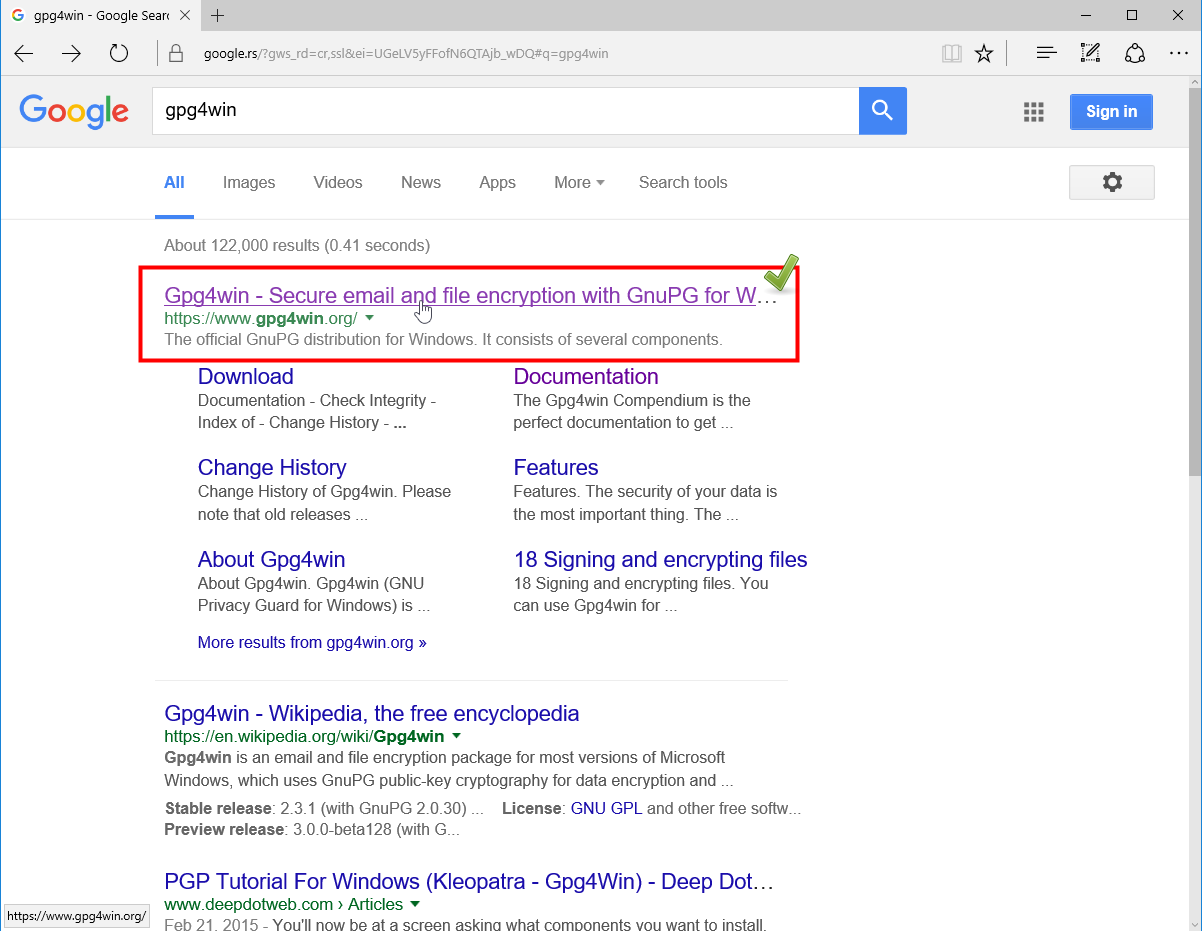
\includegraphics[width=\textwidth]{01_gpg4win_download.png}
		\caption{Preuzmite Gpg4Win sa interneta}
		\label{initialscreen}
	\end{center}
\end{figure}
\newpage
\begin{figure}[!h]
	\begin{center}
		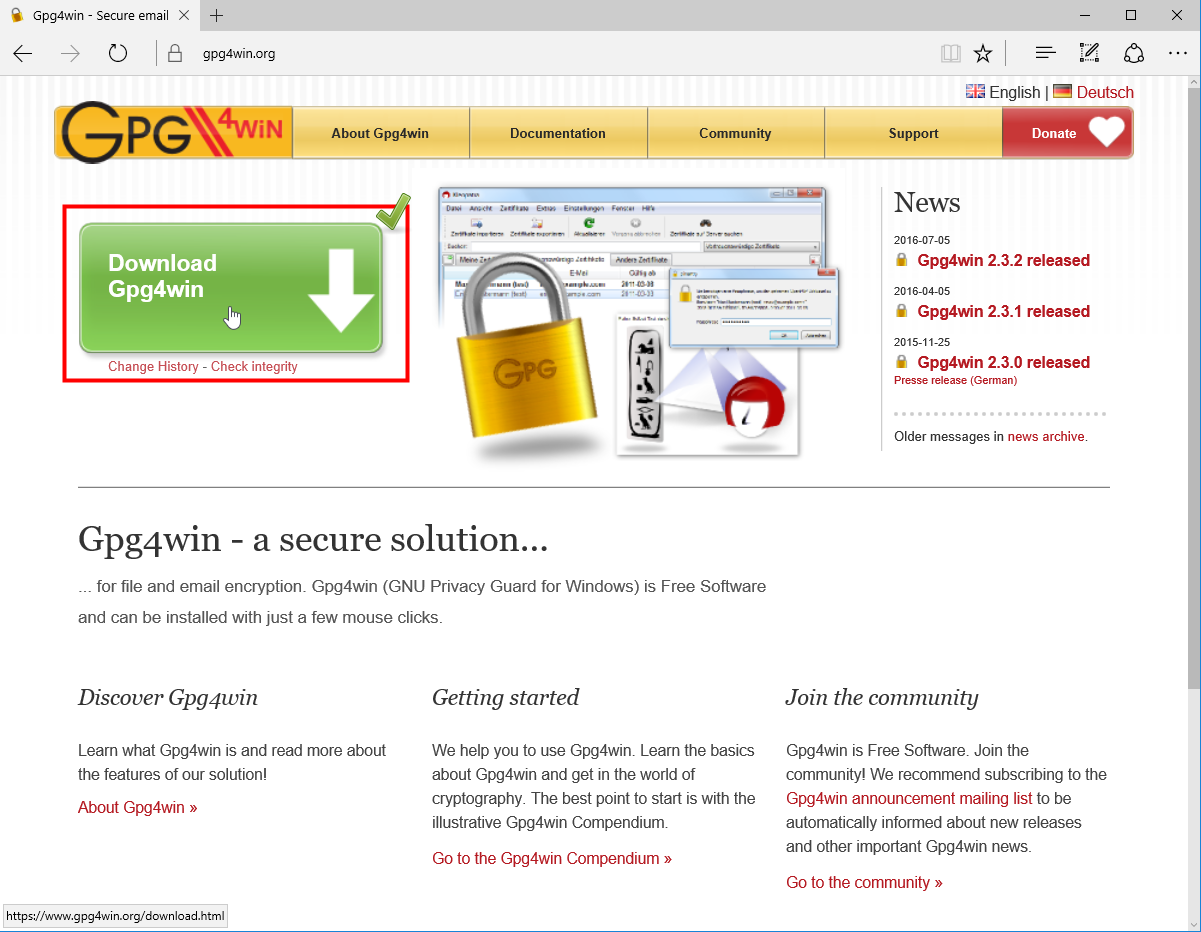
\includegraphics[width=\textwidth]{02-Gpg4win_download.png}
		\caption{Preuzmite Gpg4Win sa interneta}
		\label{initialscreen}
	\end{center}
\end{figure}
\newpage
\begin{figure}[!t]
	\begin{center}
		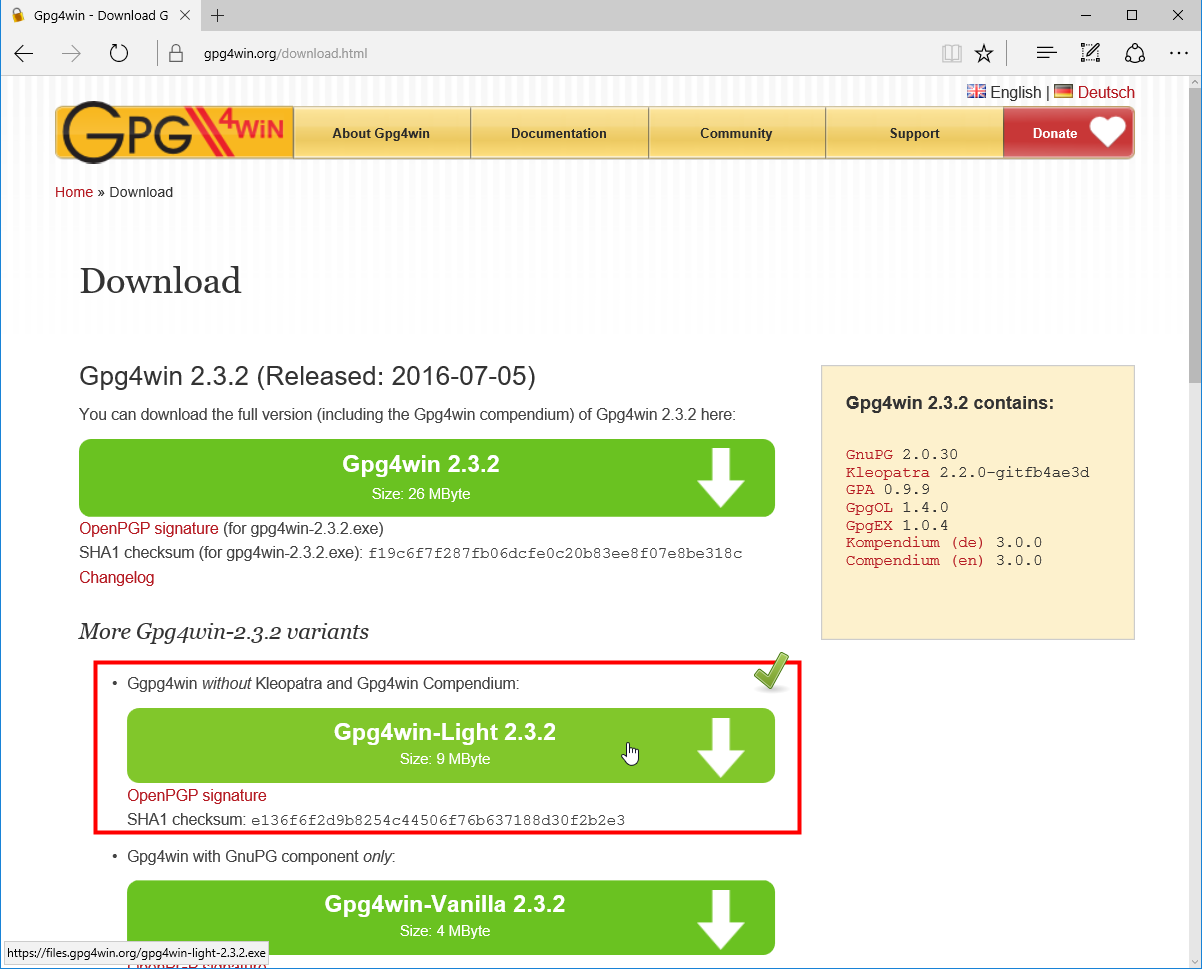
\includegraphics[width=9cm]{03_Download_Gpg4wi_Light.png}
		\caption{Odaberite Gpg4win \textbf{Light} verziju}
		\label{initialscreen}
	\end{center}
\end{figure}
Vazno je i proveriti otisak %
\footnote{Proverite digitalni otisak (he\v{s} funkciju ozna\v{c}enu kao \textbf{SHA1 checksum} na tre\'{c}oj slici) i digitalni potpis preuzetog fajla*} i digitalni potpis preuzetog programa.

\begin{figure}[!h]
	\begin{center}
		
\includegraphics[width=\textwidth]{04_Downloading_Gpg4win.png}
		\caption{sa\v{c}ekajte da se program preuzme, }
		\label{initialscreen}
	\end{center}
\end{figure}
\begin{figure}[!h]
	\begin{center}
		
\includegraphics[width=\textwidth]{05_Gpg4win_Downloaded_Gpg4win.png}
		\caption{po reuzimanju pokrenite Gpg4win program}
		\label{initialscreen}
	\end{center}
\end{figure}
\newpage
Sada samo pro\dj{}ite kroz jednostava i uobi\v{c}ajen proces intalacije Gpg4win programa, koja se svodi na kliktanje \textbf{Next} dugmeta. Instalacija je jednostavna, ali \'{c}emo svakako pro\'{c}i kroz ceo proces.
\begin{figure}[!h]
	\begin{center}
		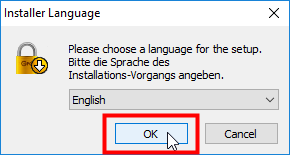
\includegraphics[width=5cm]{06_Gpg4win_Installer_Language.png}
		\caption{odaberite jezik za Gpg4win program, mi biramo Engleski}
		\label{initialscreen}
	\end{center}
\end{figure}
\begin{figure}[!h]
	\begin{center}
		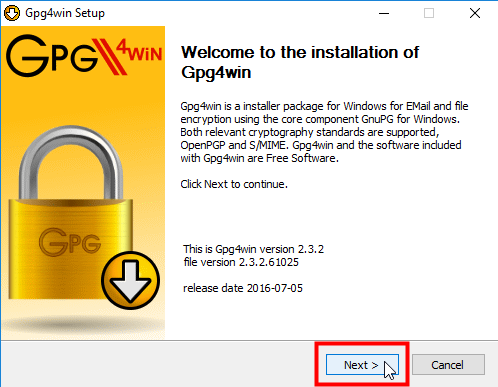
\includegraphics[width=8cm]{07_Gpg4win_Setup.png}
		\caption{Next}
		\label{initialscreen}
	\end{center}
\end{figure}
\newline
Gpg4win je slobodan softver otvorenog koda pod \textit{GNU GPL}% 
\footnote{GNU op\v{s}ta javna licenca: \href{https://goo.gl/mONh8W}{link}} licencom, tako da svako mo\v{z}e videti k\^{o}d samog softvera, uveriti se u ispravnost ili prou\v{c}avati na\v{c}in funkcionisanja istog.

\newpage
\begin{figure}[!h]
	\begin{center}
		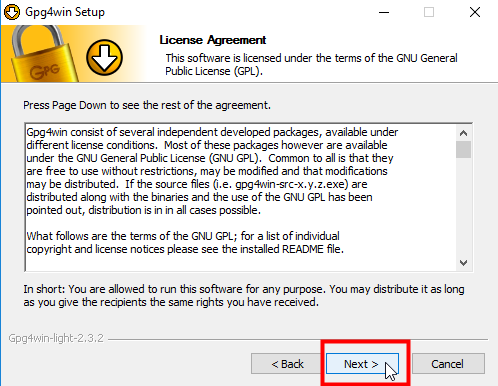
\includegraphics[width=8cm]{08_Gpg4win_Setup.png}
		\caption{Next}
		\label{initialscreen}
	\end{center}
\end{figure}
\begin{figure}[!h]
	\begin{center}
		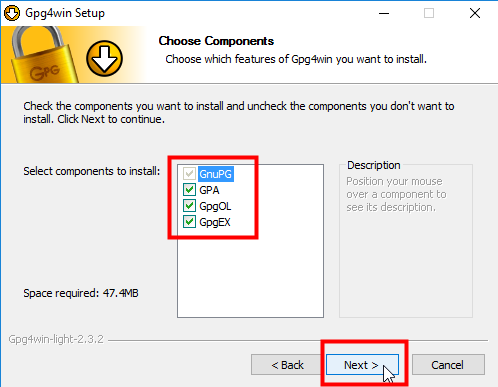
\includegraphics[width=8cm]{09_Gpg4win_Setup.png}
		\caption{Next}
		\label{initialscreen}
	\end{center}
\end{figure}
\newpage
\begin{figure}[!h]
	\begin{center}
		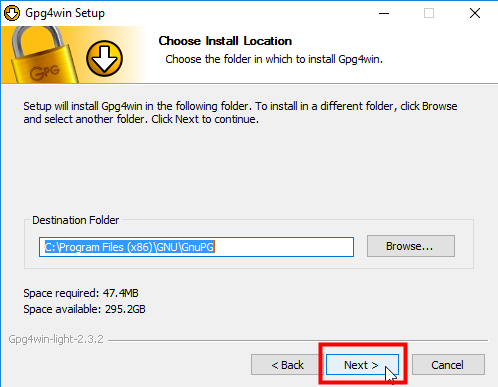
\includegraphics[width=8cm]{10_Gpg4win_Setup.png}
		\caption{Next}
		\label{initialscreen}
	\end{center}
\end{figure}
\begin{figure}[!h]
	\begin{center}
		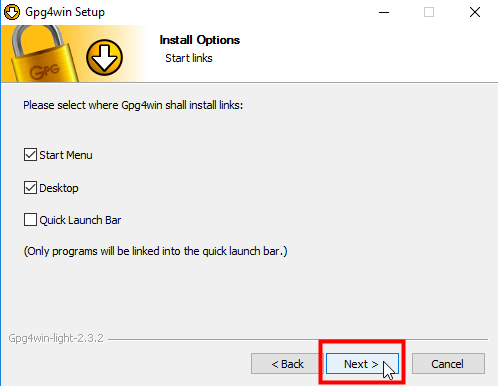
\includegraphics[width=8cm]{11_Gpg4win_Setup.png}
		\caption{Next}
		\label{initialscreen}
	\end{center}
\end{figure}
\newpage
\begin{figure}[!h]
	\begin{center}
		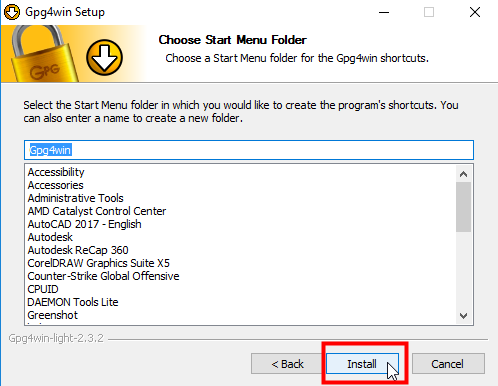
\includegraphics[width=8cm]{12_Gpg4win_Setup.png}
		\caption{Install}
		\label{initialscreen}
	\end{center}
\end{figure}
\begin{figure}[!h]
	\begin{center}
		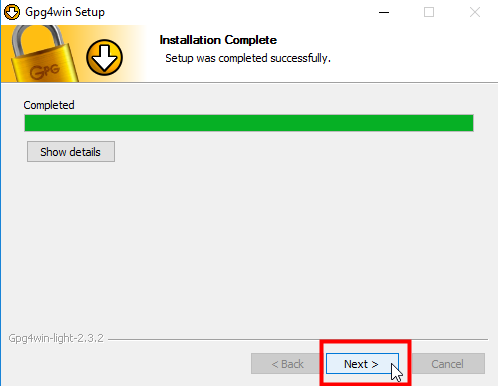
\includegraphics[width=8cm]{14_Gpg4win_Setup.png}
		\caption{Next.}
		\label{initialscreen}
	\end{center}
\end{figure}
\newpage
\begin{figure}[!h]
	\begin{center}
		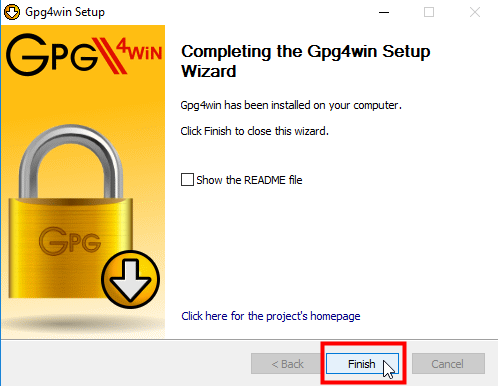
\includegraphics[width=7cm]{15_Gpg4win_Setup.png}
		\caption{Finish. Intslacija se zavr\v{s}ila}
		\label{initialscreen}
	\end{center}
\end{figure}
\begin{figure}[!h]
	\begin{center}
		
\includegraphics[width=9cm]{16_Desktop.png}
		\caption{Vide\'{c}ete ikonice na va\v{s}em Desktop-u}
		\label{initialscreen}
	\end{center}
\end{figure}
\newpage

\section{Instalacija Thunderbird programa}
Slede\'{c}i program koji nam je potreban je Thunderbird klijent elektronske po\v{s}te koga mo\v{z}ete preuzeti sa \href{https://www.mozilla.org/en-US/thunderbird/}{mozilla.org/en-US/thunderbird}.
\newline Zato preporu\v{c}ujemo \textbf{Thunderbird} klijenta elektronske po\v{s}te koji je otvorenog koda, multiplatformski, podr\v{z}ava \v{s}ifovanje elektronske po\v{s}te kroz \textbf{Enigmail} dodatak.


\begin{figure}[!h]
	\begin{center}
		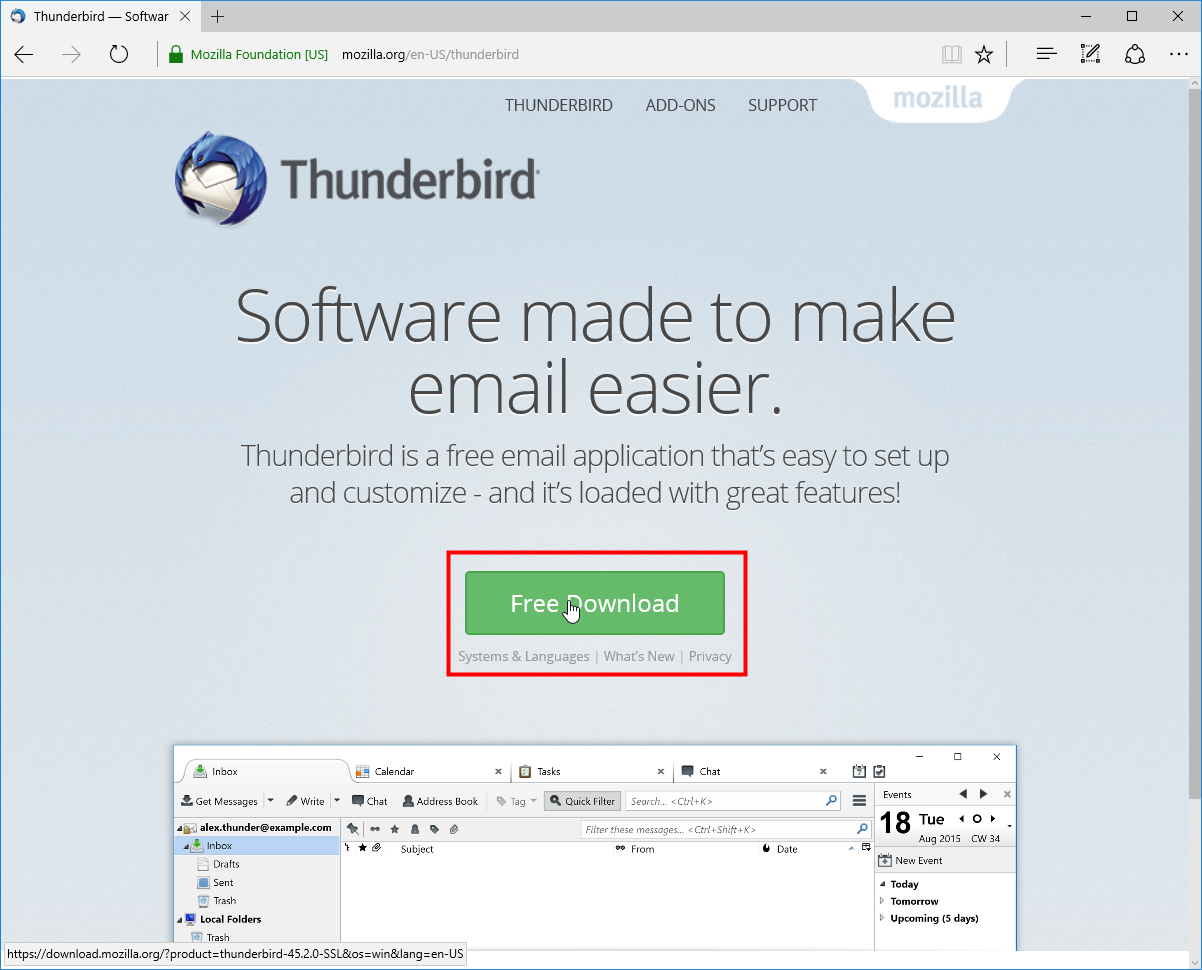
\includegraphics[width=10cm]{20_Thunderbird_Mozilla.png}
		\caption{Preuzmite Thunderbird}
		\label{initialscreen}
	\end{center}
\end{figure}
\begin{figure}[!h]
	\begin{center}
		
\includegraphics[width=\textwidth]{21_Thunderbird_Mozilla_downloading.png}
		\caption{Sa\v{c}ekajte da se zavr\v{s}i preuzimanje}
		\label{initialscreen}
	\end{center}
\end{figure}
\begin{figure}[!h]
	\begin{center}
		
\includegraphics[width=\textwidth]{22_Thunderbird_Mozilla_downloaded.png}
		\caption{Pokrenite preuzeti instalacioni fajl Thunderbird-a}
		\label{initialscreen}
	\end{center}
\end{figure}
\begin{figure}[!h]
	\begin{center}
		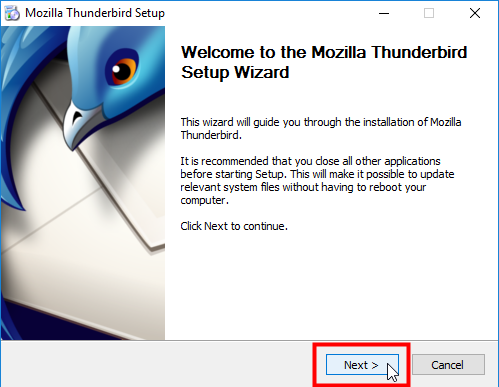
\includegraphics[width=8cm]{23_Mozilla_Thunderbird_Setup.png}
		\caption{Instalirajte thunderbird}
		\label{initialscreen}
	\end{center}
\end{figure}
\newpage
\begin{figure}[!h]
	\begin{center}
		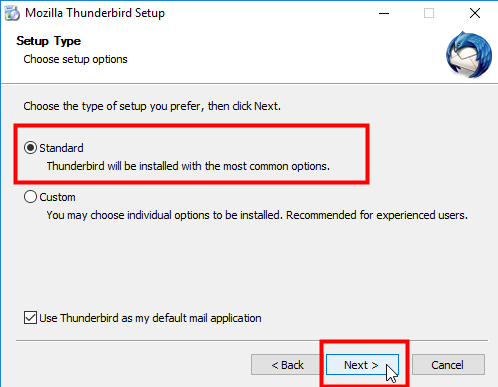
\includegraphics[width=8cm]{24_Mozilla_Thunderbird_Setup.png}
		\caption{Instalirajte Thunderbird}
		\label{initialscreen}
	\end{center}
\end{figure}
\begin{figure}[!h]
	\begin{center}
		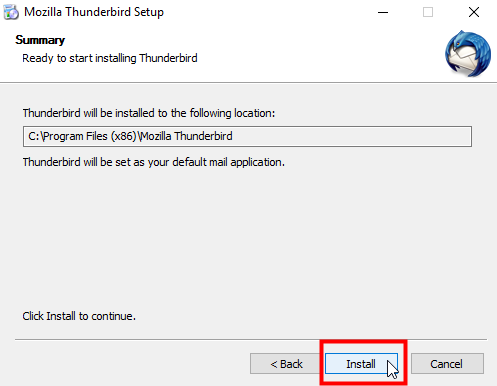
\includegraphics[width=8cm]{25_Mozilla_Thunderbird_Setup.png}
		\caption{Instalirajte Thunderbird}
		\label{initialscreen}
	\end{center}
\end{figure}
\newpage
\begin{figure}[!h]
	\begin{center}
		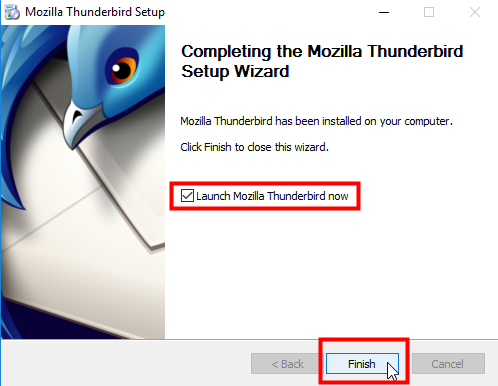
\includegraphics[width=8cm]{26_Mozilla_Thunderbird_Setup.png}
		\caption{Pokrenite Thunderbird po zavr\v{s}etku instalacije}
		\label{initialscreen}
	\end{center}
\end{figure}
\begin{figure}[!h]
	\begin{center}
		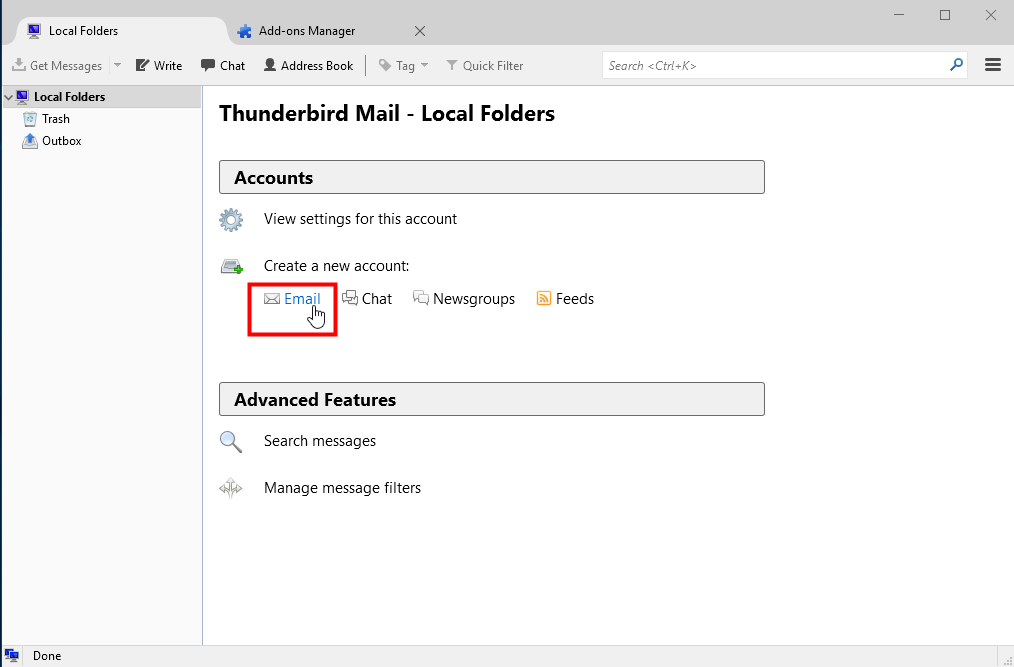
\includegraphics[width=9cm]{27_Mozilla_Thunderbird.png}
		\caption{Prvo pokretanje Thunderbird-a}
		\label{initialscreen}
	\end{center}
\end{figure}
\newpage
\begin{figure}[!h]
	\begin{center}
		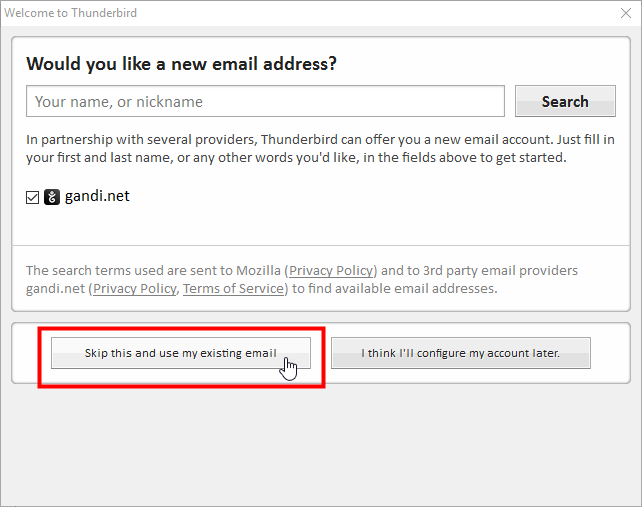
\includegraphics[width=8cm]{28_Mozilla_Thunderbird_email_setup.png}
		\caption{Odaberite da \v{z}elite da podesite va\v{s} postoje\'{c}i nalog elektronske po\v{s}te}
		\label{initialscreen}
	\end{center}
\end{figure}
\begin{figure}[!h]
	\begin{center}
		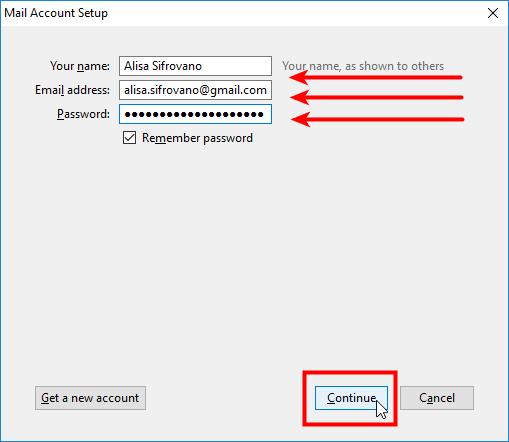
\includegraphics[width=8cm]{29_Mozilla_Thunderbird_email_credentials.png}
		\caption{Pdesite opcije za va\v{s} nalog. Na\v{s} je u ovom primeru:\newline alisa.sifrovano@gmail.com, a vi unesite va\v{s}u email adresu i sifru.}
		\label{initialscreen}
	\end{center}
\end{figure}
\newpage
\begin{figure}[!h]
	\begin{center}
		\includegraphics[width=8cm]{30_Mozilla_Thunderbird_email_credentials2.png}
		\caption{Razlika izme\dj{}u \textbf{IMAP} i \textbf{POP3} protokola je \v{s}to se kod ovog drugog po\v{s}ta \v{c}uva na va\v{s}em ra\v{c}unaru, pa u nekim slu\v{c}ajevima, Email provajder ne\'{c}e \v{c}uvati kopiju va\v{s}e po\v{s}te. }
		\label{initialscreen}
	\end{center}
\end{figure}
\newpage
\newpage
\bigskip
\subsection{instalacija Enigmail dodatka}
\begin{figure}[!h]
	\begin{center}
		\includegraphics[width=\textwidth]{31_Mozilla_Thunderbird_plugins.png}
		\caption{Izaberimo opciju "Add-ons" iz Thunderbird-a kako bi smo instalirali \textbf{Enigmail}}
		\label{initialscreen}
	\end{center}
\end{figure}

Sada je i \textbf{Thunderbird} mejl klijent instaliran, pode\v{s}ena \v{z}eljena adresa, pa prelazimo na instalaciju 
\textbf{Enigmail} dodatka (eng. Add-ons) mejl klijentu koji \'{c}e nam omogu\'{c}iti \v{s}ifrovanje/de\v{s}ifrovanje, digitalno potpisivanje i provere digitalnih potpisa iz samog mejl klijenta.
\newline Enigmail pru\v{z}a pomenute funkcionalnost kroz koriste\'{c}i predhodno instaliran \textbf{Gpg4win}, tako da ne morate da pokre\'{c}ete \textbf{Gpg4Win} (\textbf{GPA} ikonica na desktop-u), nego pomenute operacije izvodite direktno iz \textbf{Thunderbird}-a. \newline
\textbf{Enigmail} je dobro integrisan u \textbf{Thunderbird} tako da mo\v{z}e da upamti va\v{s}u \v{s}ifru za privatni klju\v{c}, automatksi de\v{s}ifruje nove poruke po prispe\'{c}u, proverava digitalni potpis i vizuelno signalizira ispravnost istih razli\v{c}itim bojama.
\newpage
\begin{figure}[!h]
	\begin{center}
		\includegraphics[width=\textwidth]{32_Addons_Manager_Mozilla_Thunderbird.png}
		\caption{Tra\v{z}imo \textbf{Enigmail} dodatak}
		\label{search_for_enigmail}
	\end{center}
\end{figure}

\begin{figure}[!h]
	\begin{center}
		\includegraphics[width=\textwidth]{33_Addons_Manager_Mozilla_Thunderbird.png}
		\caption{Posle instaliranja \textbf{Enigmail}-a restartujemo \textbf{Thunderbird}}
		\label{restart_thunderbird}
	\end{center}
\end{figure}
\newpage
\subsection{Generisanje GPG klju\v{c}eva}
\begin{figure}[!h]
	\begin{center}
		\includegraphics[width=\textwidth]{34_Enigmail_option.png}
		\caption{Sada trebamo da generi\v{s}emo \textbf{GPG} klju\v{c}ece u \textbf{Enigmail}-u}
		\label{enigmail_setup_wizard}
	\end{center}
\end{figure}

\begin{figure}[!h]
	\begin{center}
		\includegraphics[width=8cm]{35_Enigmail_Setup_Wizard.png}
		\caption{Pokrenite \textbf{Wizard} izaberite \texttt{standardni} na\v{c}in konfigurisanja .}
		\label{enigmail_setup_wizard2}
	\end{center}
\end{figure}
\newpage
\begin{figure}[!h]
	\begin{center}
		\includegraphics[width=9cm]{36_Enigmail_Setup_Wizard.png}
		\caption{\textbf{Wizard} \'{c}e prepoznati predhodno pode\v{s}en mejl nalog.
		\newline Vi samo treba da podesite \v{s}ifru za va\v{s}e nove \textbf{GPG} klju\v{c}eve koji \'{c}e \textbf{Wizard} generisati za vas.}
		\label{enigmail_setup_wizard3}
	\end{center}
\end{figure}

\begin{figure}[!h]
	\begin{center}
		\includegraphics[width=9cm]{37_Enigmail_Setup_Wizard.png}
		\caption{Sa\v{c}ekajte da \textbf{Wizard} generi\v{s}e nove \textbf{GPG} klju\v{c}eve za vas.}
		\label{enigmail_setup_wizard4}
	\end{center}
\end{figure}
\newpage
\begin{figure}[!h]
	\begin{center}
		\includegraphics[width=9cm]{38_Enigmail_Setup_Wizard.png}
		\caption{Kada se generisanje klju\v{c}eva zavr\v{s}i, ponudi\'{c}e vam da generi\v{s}ete \textsf{Sertifikat za opoziv klju\v{c}eva} (eng. Revocation certificate), obavezno to i u\v{c}inite}
		\label{enigmail_setup_wizard5}
	\end{center}
\end{figure}

\begin{figure}[!h]
	\begin{center}
		\includegraphics[width=9cm]{39_Enigmail_Setup_Wizard.png}
		\caption{Naravno, morate uneti i \v{s}ifru za \textbf{GPG} klju\v{c} koju ste malopre podesili}
		\label{enigmail_setup_wizard6}
	\end{center}
\end{figure}
\newpage
\begin{figure}[!h]
	\begin{center}
		\includegraphics[width=11cm]{40_Create_&_Save_Revocation_Certificate.png}
		\caption{Sa\v{c}uvajte sertifikat za opoziv klju\v{c}eva.}
		\label{enigmail_setup_wizard7}
	\end{center}
\end{figure}

\begin{figure}[!h]
	\begin{center}
		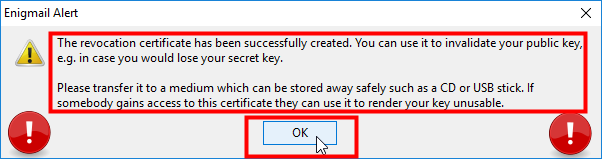
\includegraphics[width=9cm]{41_Enigmail_Alert.png}
		\caption{Napravite bekap kopiju na neki USB jer ovaj sertifikat treba da \v{c}uvate u tajnosti.
		\newline Ovaj sertifikat \'{c}e vam omogu\'c{}iti da opozovete va\v{s}e klju\v{c}eve, ukoliko ih izgubite.}
		\label{enigmail_setup_wizard8}
	\end{center}
\end{figure}
\newpage
\begin{figure}[!h]
	\begin{center}
		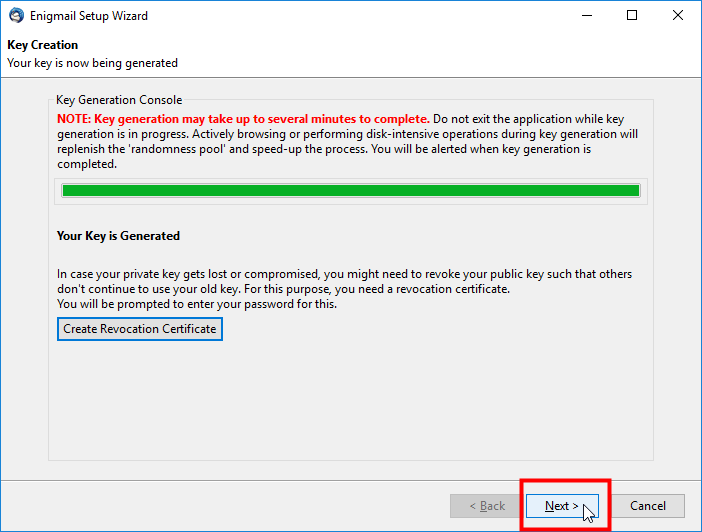
\includegraphics[width=9cm]{42_Enigmail_Setup_Wizard.png}
		\caption{Nstavite sa procesom.}
		\label{enigmail_setup_wizard9}
	\end{center}
\end{figure}

\begin{figure}[!h]
	\begin{center}
		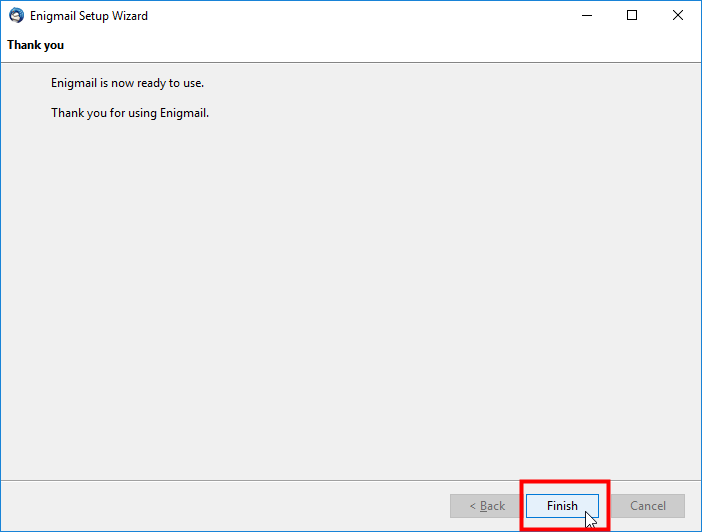
\includegraphics[width=9cm]{43_Enigmail_Setup_Wizard.png}
		\caption{Zavr\v{s}ite sa procesom generisanja klju\v{c}eva.}
		\label{enigmail_setup_wizard10}
	\end{center}
\end{figure}
\newpage
\section{Slanje javnog klju\v{c}a na server javnih klju\v{c}eva}

\begin{figure}[!h]
	\begin{center}
		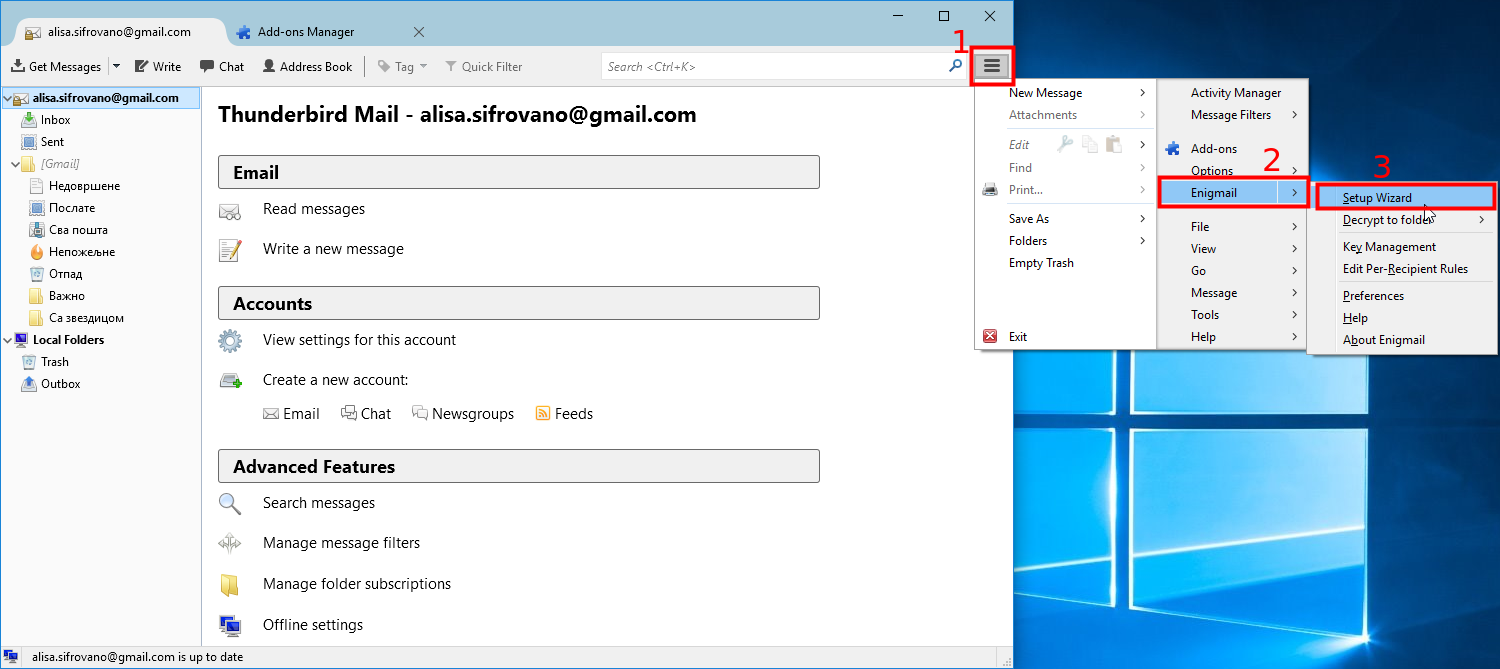
\includegraphics[width=\textwidth]{44_Enigmail_Setup_Wizard.png}
		\caption{Sada je potrebno da po\v{s}aljemo na\v{s} javni klju\v{c} na server javnih klju\v{c}eva kako bi ostali mogli da lako prona\dj{}u na\v{s} javni klju\v{c} i njime \v{s}ifruju poruku za nas.}
		\label{uploading_pubkey_enigmail}
	\end{center}
\end{figure}

\begin{figure}[!h]
	\begin{center}
		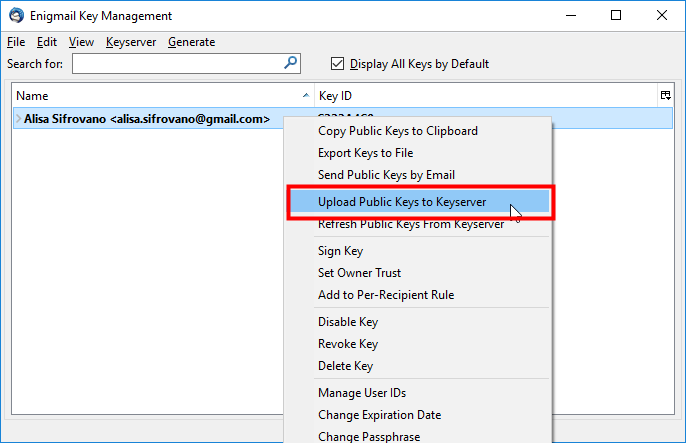
\includegraphics[width=9cm]{45_Enigmail_Key_Management.png}
		\caption{Slanje klju\v{c}eva naravno obavljamo iz \textbf{Enigmail}-a}
		\label{uploading_pubkey_enigmail2}
	\end{center}
\end{figure}
\newpage
\section{Razmena \v{s}ifrovanih poruka}
\subsection{Nabavka javnog klju\v{c}a sagovornika}

\begin{figure}[!h]
	\begin{center}
		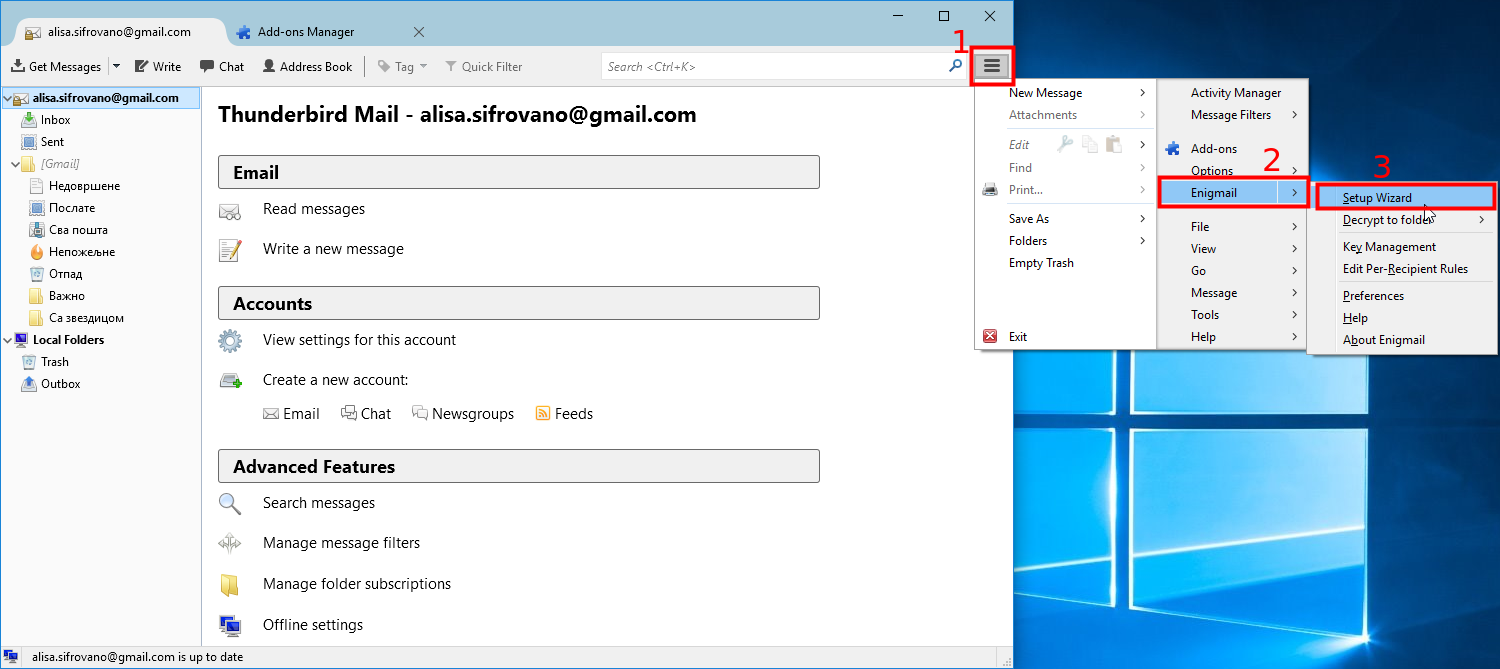
\includegraphics[width=\textwidth]{44_Enigmail_Setup_Wizard.png}
		\caption{Da bi smo poslali \v{s}ifrovanu poruku nekome moramo imati javni klju\v{c} te osobe, tj. i ta osoba mora    koristiti \textbf{GPG}}
		\label{search_for_pubkey}
	\end{center}
\end{figure}

\begin{figure}[!h]
	\begin{center}
		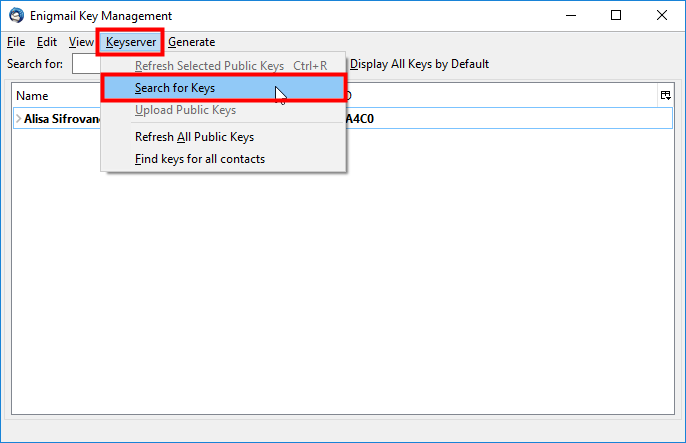
\includegraphics[width=9cm]{47_keymanagment_searchforkey.png}
		\caption{Tra\v{z}enje javnog klju\v{c}a osobe kojoj \v{z}elimo poslati \v{s}ifrovanu poruku.}
		\label{search_for_pubkey2}
	\end{center}
\end{figure}
\newpage
\begin{figure}[!h]
	\begin{center}
		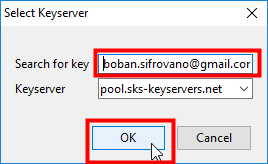
\includegraphics[width=5cm]{48_keymanagment_searchforkey.png}
		\caption{Klju\v{c} tra\v{z}imo po mejl adresi}
		\label{search_for_pubkey3}
	\end{center}
\end{figure}

\begin{figure}[!h]
	\begin{center}
		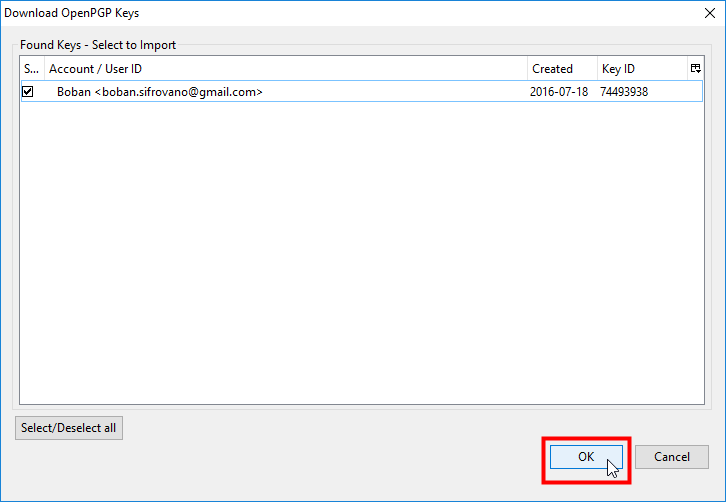
\includegraphics[width=9cm]{49_keymanagment_searchforkey.png}
		\caption{I ako je druga osoba napravila svoj klju\v{c} i poslala ga na server, kao \v{s}to smo to i mi uradili, klju\v{c} \'{c}e biti prona\dj{}en}
		\label{search_for_pubkey4}
	\end{center}
\end{figure}
\newpage
\begin{figure}[!h]
	\begin{center}
		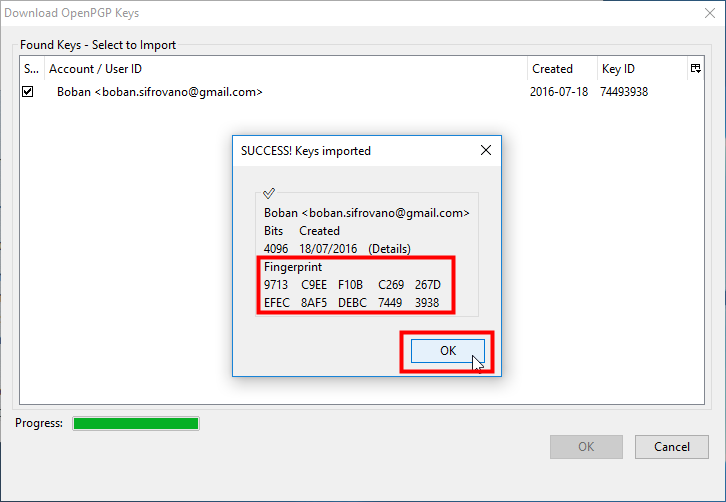
\includegraphics[width=9cm]{50_keymanagment_searchforkey.png}
		\caption{Bi\'{c}e jedinstvani prikazan i otisak klju\v{c} (eng. Fingerprint)}
		\label{search_for_pubkey5}
	\end{center}
\end{figure}

\begin{figure}[!h]
	\begin{center}
		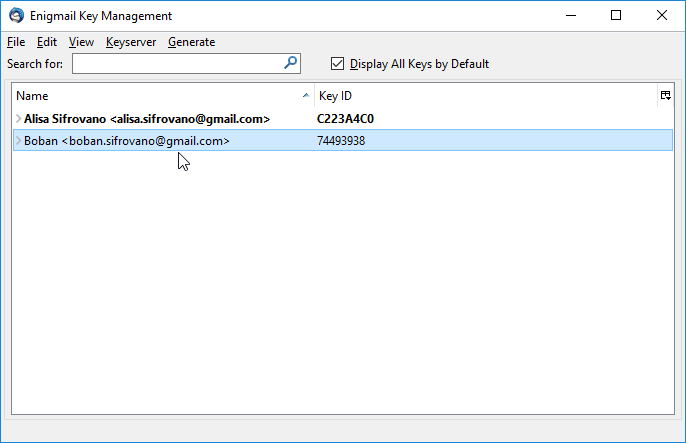
\includegraphics[width=9cm]{51_keymanagment_searchforkey.png}
		\caption{I klju\v{c} \'{c}e biti u va\v{s}oj bazi klju\v{c}eva.\newline Ceo ovaj proces nabavke klju\v{c}a je potrebno uraditi samo jednom za svaku osobu sa kojom \v{z}elite da razmenjujete \v{s}ifrovane poruke.}
		\label{search_for_pubkey6}
	\end{center}
\end{figure}
\newpage
\subsection{Slanje \v{s}ifrovane poruke}
\begin{figure}[!h]
	\begin{center}
		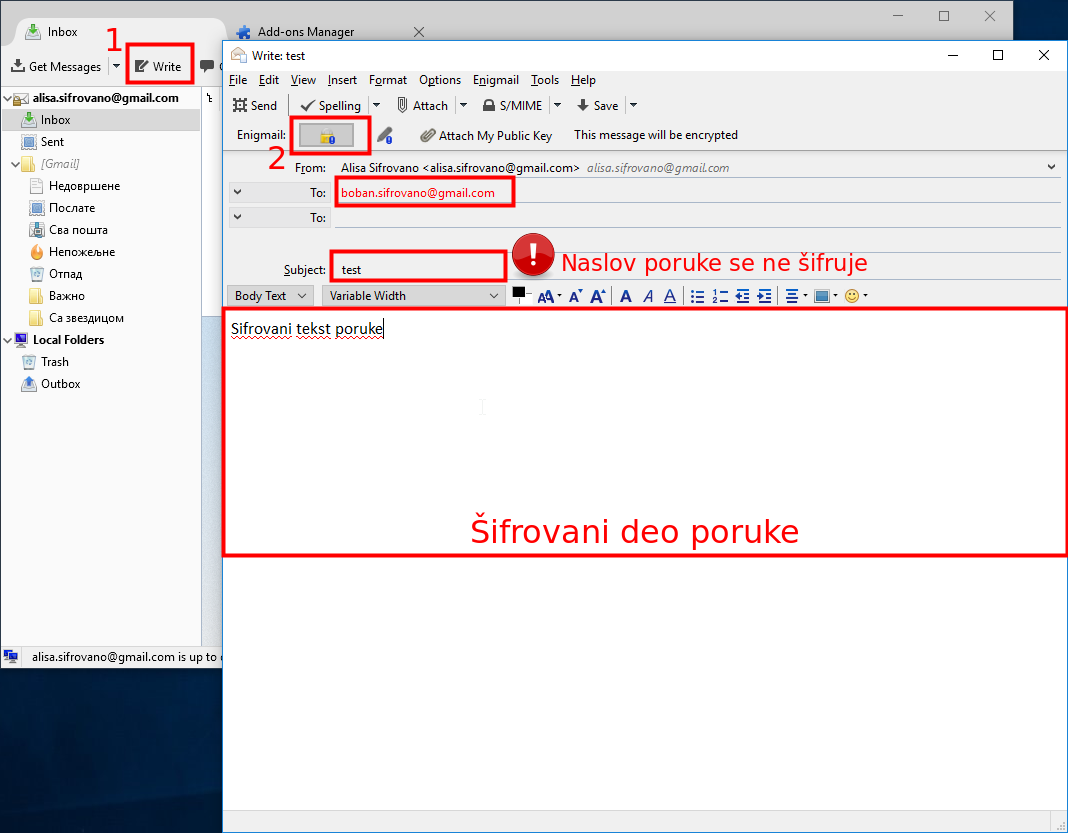
\includegraphics[width=8cm]{52_write_encrypted_message.png}
		\caption{Sastavimo novu \v{s}ifrovanu poruku za Bobana (boban.sifrovano@gmail.com)\newline Mala napomena da \textbf{GPG} \v{s}ifruje samo "telo" poruke, ne i naslov!}
		\label{compose_message}
	\end{center}
\end{figure}
\begin{figure}[!h]
	\begin{center}
		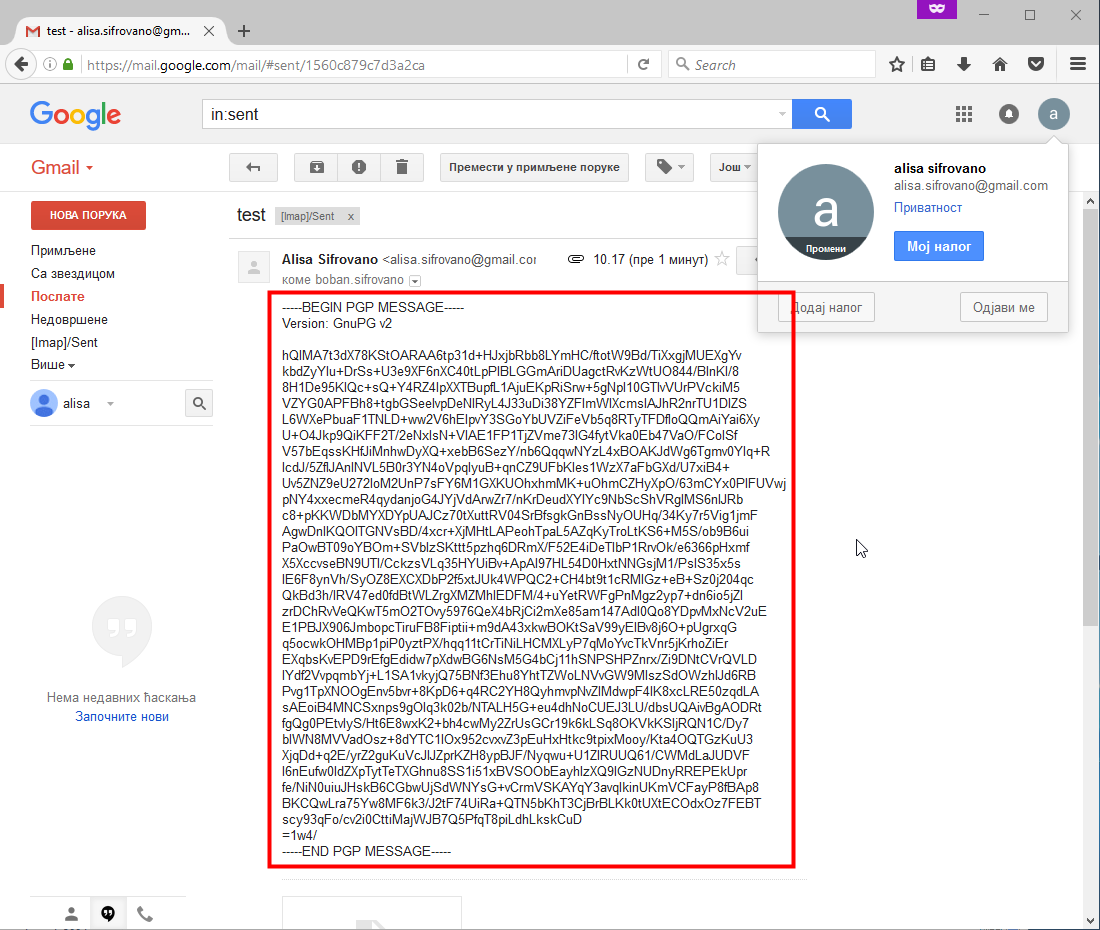
\includegraphics[width=8cm]{53_encrypted_message_google.png}
		\caption{Kada razmenjujemo \v{s}ifrovane poruke, sve \v{s}te na\v{s} mejl provajder vidi je \v{s}ifrovana poruka, naslov poruke, i kome je poruka upu\'{c}ena. \newline\newline\newline}
		\label{Email_provider_sees_encrypted_message}
	\end{center}
\end{figure}
\newpage

\subsection{De\v{s}ifrovanje primljenje \v{s}ifrovane po\v{s}te}
\begin{figure}[!h]
	\begin{center}
		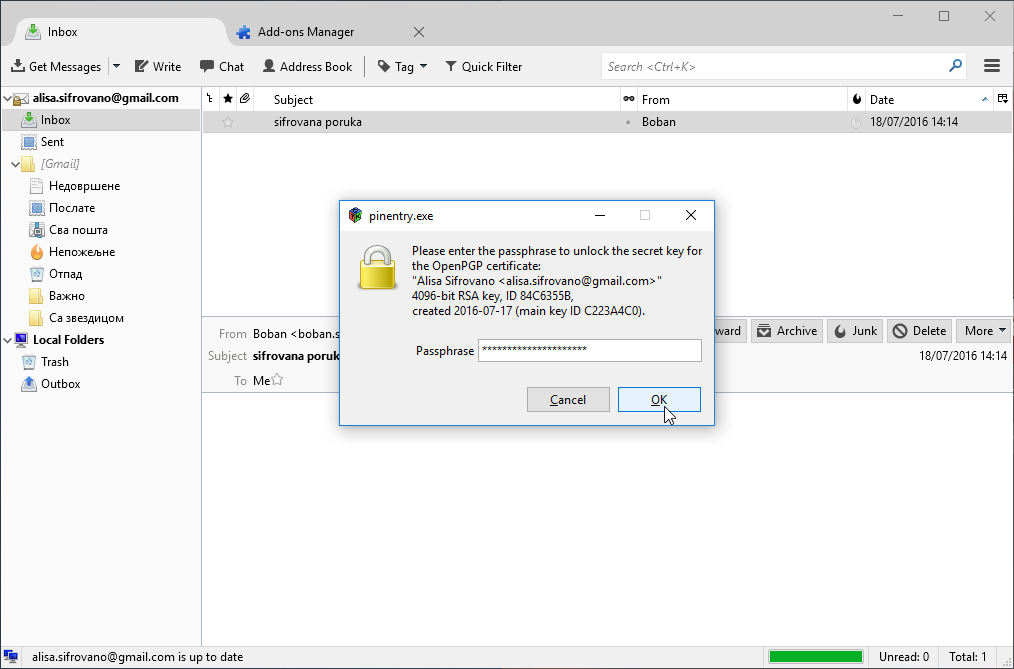
\includegraphics[width=9cm]{Inbox_decrypt1.png}
		\caption{Kada dobijete \v{s}ifrovanu poruku, \textbf{Enigmail} \'{c}e vam tra\v{z}iti \textbf{GPG} \v{z}ifru da bi ste de\v{s}ifrovali mejl.}
		\label{Email_provider_sees_encrypted_message}
	\end{center}
\end{figure}

\begin{figure}[!h]
	\begin{center}
		\includegraphics[width=9cm]{Inbox_decrypt2.png}
		\caption{Po uno\v{s}enju \v{s}ifre, vide\'{c}ete originalni tekst de\v{s}ifrovane poruke.}
		\label{Email_provider_sees_encrypted_message}
	\end{center}
\end{figure}
\newpage
\section{Dodatak}
\subsection{Windows Live Mail}
Iako na Windows-u ve\'{c} postoji \textsf{Windows Live Mail} on ne podr\v{z}ava \v{s}ifrovanje elektronske po\v{s}te
niti postoje dodaci (eng. plugins) koji bi tu funkcionalnost omogu\'{c}ili u Windows Live Mail-u.
Tako\dj{}e, Windows Live Mail je vlasni\v{c}ki softver zatvorenog koda, pa ne bi trebalo da imate poverenja u njega i iz tog razloga.
Me\dj{}utim, ako se iz nekog razloga \v{z}elite ostati pri \textsf{Windows Live Mail}-u, a u isto vreme \v{z}elite razmenjivati \v{s}ifrovane poruke, to mo\v{z}ete u\v{c}initi kombinovanjem predhodno instaliranog \textbf{Gpg4Win} tj. \textbf{GPA} programa. Naime, GPA ima \textsc{Clipboard} prozor u kome mo\v{z}ete uneti tekst koji potom pritiskom na dugme \textsc{Encrypt} \v{s}ifrujete poruku, pritiskom na dugme \textsc{Sign} digitalno potpisujete poruku. Kada poruku \v{s}ifrujete u \textbf{GPA} programu onda je samo prekopirate u \textsf{Windows Live Mail} u prozoru gde bi ste ina\v{c}e sastavljali poruku, i zatim samo po\v{s}aljete.
\newpage
\begin{figure}[!h]
	\begin{center}
		\includegraphics[width=9cm]{wlm_GPA.png}
		\caption{Pokrenite \textbf{GPA}}
		\label{gpa_WLM1}
	\end{center}
\end{figure}

\begin{figure}[!h]
	\begin{center}
		\includegraphics[width=9cm]{wlm_GPA_clipboard2.png}
		\caption{Otvori\'{c}e vam se \textbf{Clipboard} u kome mo\v{z}ete sastaviti poruku,\newline a potom pritisnite \textbf{Encrypt} dugme.}
		\label{gpa_WLM2}
	\end{center}
\end{figure}
\bigskip
\bigskip
\newpage
\begin{figure}[!h]
	\begin{center}
		\includegraphics[width=6cm]{wlm_GPA_clipboard_encrypt.png}
		\caption{Zati \'{c}e se otvoriti prozor u kome treba da odaberete klju\v{c} tj. mejl primaoca za koga \v{s}ifrujete poruku.\newline Ovo podrazumeva da ste  predhodno uvezli primao\v{c}ev javni klju\v{c}.}
		\label{gpa_WLM3}
	\end{center}
\end{figure}

\begin{figure}[!h]
	\begin{center}
		\includegraphics[width=9cm]{wlm_GPA_clipboard4.png}
		\caption{Proverite i potvrdite akciju \v{s}ifrovanja.}
		\label{gpa_WLM4}
	\end{center}
\end{figure}
\newpage
\begin{figure}[!h]
	\begin{center}
		\includegraphics[width=9cm]{wlm_GPA_clipboard5_copy_message.png}
		\caption{Tekst poruke \'{c}e se zatim \v{s}ifrovati, a vi ga \v{s}ifrovanog trebate prekopirati u Windows Live Mail u polje za sastavljanje nove poruke}
		\label{gpa_WLM5}
	\end{center}
\end{figure}

\begin{figure}[!h]
	\begin{center}
		\includegraphics[width=11cm]{EncryptedMailWLM.png}
		\caption{Kada prekopirate \v{s}ifrovani tekst u Windows Live Mail unesite primaoca (onog istog za koga ste \v{s}ifrovali poruku), i po\v{s}aljite je.}
		\label{gpa_WLM6}
	\end{center}
\end{figure}


\end{document}